%%================================================
%% Filename: main.tex
%% Encoding: UTF-8
%% Author: Yuan Xiaoshuai - yxshuai@gmail.com
%% Created: 2012-01-08 13:09
%% Last modified: 2020-04-05 21:01
%%================================================
\documentclass[doctor]{htuthesis}
% 自定义宏包
\usepackage{docutils}

% 图形文件路径
\graphicspath{{figures/}}

\begin{document}

% 封面、目录、符号对照表等
\frontmatter

%%================================================
%% Filename: cover.tex
%% Encoding: UTF-8
%% Author: Yuan Xiaoshuai - yxshuai@gmail.com
%% Created: 2012-01-14 13:44
%% Last modified: 2019-11-03 00:30
%%================================================
% 研究生论文：单位代码、学号或申请号、分类号（真值来源：参考论文 PDF page 2 + .doc 空白模板）
% 分类号依《中国图书馆图书分类法》（第五版）检索（spec §1.1.1）
\schoolcode{10476}
\id{208010102893000753}
\secretlevel{D669.3}

% 论文题目
\ctitle{河南师范大学学位论文 \LaTeX\ 模板使用示例}

% 研究生论文：
% 学科、专业（封面合并为一行）、研究方向、申请学位类别、申请人、指导教师
% 学科、专业 以国务院学位委员会《研究生教育学科专业目录》（2022）为准（spec §1.1.1）
\csubject{政治学}
\cmajor{政治学理论}
\researchdirection{社区治理}
\degreecategory{法学博士}
\cauthor{赵钱孙}
\csupervisor{吴郑王}
\protitle{教授}%
\stuno{20080800901}%本科论文需要学号（博士封面不渲染，保留无害）
% 时间自动生成（阿拉伯数字+年/月；.doc 空白模板 + 参考论文双源确认）
% \cdate{\CJKdigits{\the\year}年\CJKnumber{\the\month}月}
% \cdate{2012年6月}

% 研究生论文：英文封面
\etitle{An Introduction to \LaTeX{} Thesis Template of Henan Normal University}
\emajor{Materials Science and Engineering}
\edepartment{School of Materials Science and Engineering}
\eauthor{Zhao Qiansun}
\esupervisor{Prof. Wu Zhengwang}
% \edate{December, 2005}%英文日期自动生成
%封面
\input{data/abstract}%摘要
\makecover

\tableofcontents%目录

\listoffigures%插图清单
\listoftables%表格清单

\makeatletter%符号对照表
  \include{data/denotation}
\makeatother

% 正文部分
\mainmatter
\include{data/chap01}
\include{data/chap02}
\include{data/chap03}
\include{data/chap04}

% 参考文献、致谢、附录等
\backmatter

% 参考文献（Story 3.12 Option A — biblatex GB/T 7714-2015 双模式 §2.14 case-2）
% \makebibliography 按文献类型分节重组（引文脚注 + 文末表；cls 定义）
\makebibliography

% 附录（spec §2.15；Story 4.1 接入 — 首次编译验证 G5a 正文小四宋体 + G5b 图A-1 counter + G3 sc 模式）
%   后置顺序：参考文献 → 附录 → 致谢 → 个人简历 → 声明（spec §1.1 结尾部分）。
\appendix
%%================================================
%% Filename: app01.tex
%% Encoding: UTF-8
%% Author: Yuan Xiaoshuai - yxshuai@gmail.com
%% Created: 2012-04-25 15:16
%% Last modified: 2019-11-07 12:55
%%================================================
\chapter{表格附件}
% 替换相应表格即可

% [Story 4.1] 附录样本浮动体 — 首次编译触发 G5b 附录编号 图A-1 / 表A-1 / （A-1）
%   （\appendix → \thechapter=Alph → \thefigure/\thetable/\theequation 呈 A-1 形式；HTU §2.11/§2.12/§2.13）。
%   示例内容（非模板标识，test-design-epic-4「Not in Scope」：样本 verbatim 保真出范围）；验证附录 counter 机制。
\section*{附录浮动体编号示例}
\addcontentsline{toc}{section}{附录浮动体编号示例}

附录中的浮动体编号沿用附录章字母前缀。如附录图~\ref{fig:app-demo}、附录表~\ref{tab:app-demo}、
附录公式~\eqref{eq:app-demo} 所示，编号形式为 A-1。

\begin{figure}[htbp]
  \centering
  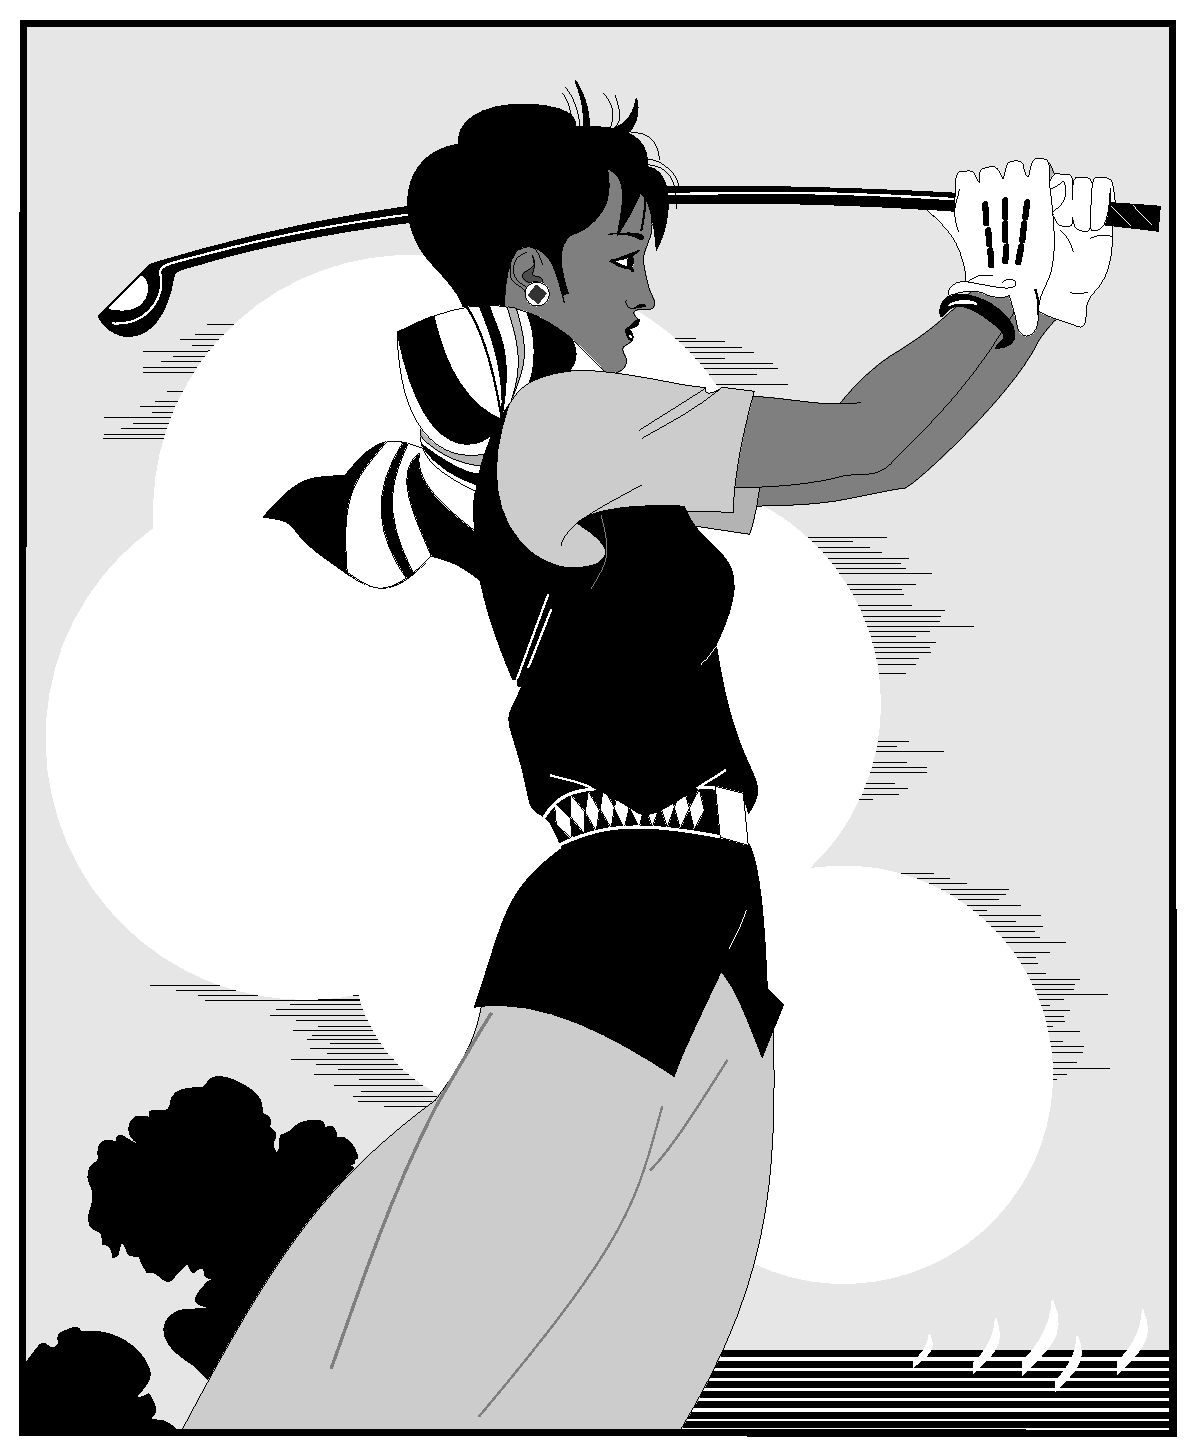
\includegraphics[width=0.5\textwidth]{golfer}
  \caption{附录示例图}\label{fig:app-demo}
\end{figure}

\begin{table}[htbp]
  \centering
  \caption{附录示例表}\label{tab:app-demo}
  \begin{tabular}{cc}
    \hline
    项目 & 数值 \\
    \hline
    A & 1 \\
    B & 2 \\
    \hline
  \end{tabular}
\end{table}

\begin{equation}\label{eq:app-demo}
  E = m c^{2}
\end{equation}

\clearpage
\section*{毕业设计（论文）任务书}
\addcontentsline{toc}{section}{附表~1：毕业设计（论文）任务书}

\clearpage
\section*{河南师范大学毕业论文开题报告表}
\addcontentsline{toc}{section}{附表~2：河南师范大学毕业论文开题报告表}

\clearpage
\section*{毕业设计（论文）计划进程表}
\addcontentsline{toc}{section}{附表~3：毕业设计（论文）计划进程表}

\clearpage
\section*{河南师范大学毕业设计中期检查表}
\addcontentsline{toc}{section}{附表~4：河南师范大学毕业设计中期检查表}

\clearpage
\section*{毕业设计（论文）成绩评定表}
\addcontentsline{toc}{section}{附表~5：毕业设计（论文）成绩评定表}
\include{data/app02}
\include{data/app03}

% 研究论文：致谢
\include{data/ack}

% 个人简历
\include{data/resume}

% 原创性声明和授权说明（结尾部分末项，spec §1.1；FR-14）
\makedeclaration

\end{document}
